% ============================================================
%  LEMBAR SOAL  --  FISIKA  --  SSU-ITB 2026  |  Paket 8
%  Sumber: SM ITB 2023 (30 soal Fisika)
% ============================================================

\documentclass[11pt]{article}
\usepackage[utf8]{inputenc}
\usepackage[T1]{fontenc}
\usepackage[a4paper,margin=2.5cm,top=2.8cm]{geometry}
\usepackage{amsmath,amssymb}
\usepackage{graphicx}
\usepackage{enumitem}
\usepackage{multicol}
\usepackage{xcolor}
\usepackage[most]{tcolorbox}
\usepackage{fancyhdr}
\usepackage{booktabs}
\usepackage{icomma}
\usepackage{array}

\definecolor{mapelcolor}{RGB}{20,70,150}
\definecolor{mapelbg}{RGB}{230,238,255}

\pagestyle{fancy}\fancyhf{}
\lhead{\small SSU-ITB 2026 --- Fisika}
\rhead{\small Paket 8}
\cfoot{\small\thepage}
\renewcommand{\headrulewidth}{0.4pt}

\newtcolorbox{soal}[1]{
  breakable,
  colback=white, colframe=black!70,
  coltitle=white, colbacktitle=black,
  fonttitle=\bfseries\sffamily,
  title=Nomor #1,
  boxrule=0.8pt, arc=3pt,
  left=3mm, right=3mm, top=2mm, bottom=2mm}

\newenvironment{pil}{%
  \begin{enumerate}[label=(\alph*),leftmargin=*,itemsep=1pt,topsep=3pt]}%
  {\end{enumerate}}
\newenvironment{pilB}{%
  \par\smallskip\begin{multicols}{2}
  \begin{enumerate}[label=(\alph*),leftmargin=*,itemsep=1pt,topsep=3pt]}%
  {\end{enumerate}\end{multicols}}

\newcommand{\gambar}[2][0.52\textwidth]{%
  \begin{center}\includegraphics[width=#1]{#2}\end{center}}

\linespread{1.05}

\begin{document}
\thispagestyle{empty}

\begin{center}
  \fbox{\parbox{0.6\textwidth}{\centering\bfseries\large LEMBAR SOAL}}
\end{center}
\vspace{0.5cm}

\begin{center}
  {\LARGE\bfseries FISIKA}
\end{center}
\vspace{0.5cm}

\begin{center}
  \begin{tabular}{ll@{\hspace{0.4cm}:@{\hspace{0.4cm}}}l}
    & Jenjang      & SMA / Sederajat               \\[0.3em]
    & Hari/Tanggal & \underline{\hspace{5cm}}      \\[0.3em]
    & Waktu        & \underline{\hspace{5cm}}      \\[0.3em]
    & Paket Soal   & 8                             \\
  \end{tabular}
\end{center}

\vspace{0.4cm}
\noindent\rule{\linewidth}{0.6pt}
\vspace{0.2cm}

\noindent\textbf{\underline{PETUNJUK UMUM}}
\begin{enumerate}[leftmargin=*,itemsep=4pt,topsep=4pt]
  \item Anda \textbf{tidak} diperbolehkan menggunakan sumber-sumber eksternal,
        termasuk internet, \textit{large language model} seperti ChatGPT, Claude,
        LLaMA, Gemini, Meta AI, dan sebagainya. Anda sangat dianjurkan untuk
        mencoba mengerjakan sendiri terlebih dahulu karena evaluasi ini dibuat
        untuk \textbf{mengukur} tingkat kepahaman; nilai $<70$ mengindikasikan
        \textbf{tidak lulus}, dan jika sudah melewati \textit{deadline} maka
        dianggap tidak mengerjakan yang berarti \textbf{tidak lulus}.

  \item Terdapat 2 tahap pengerjaan, yaitu tahap \textbf{Try Out} dan tahap
        \textbf{Review}. Try Out bersifat \textit{open book}; Anda diperbolehkan
        membuka buku apapun selama bersifat \textit{offline} dengan rentang waktu
        2 jam pada tanggal \underline{\hspace{3cm}}. Setelah itu memasuki
        tahap Review dengan \textit{schedule} rentang tanggal
        \underline{\hspace{3cm}}--\underline{\hspace{3cm}}, di mana Anda
        diharapkan mengerjakan ulang dengan disertakan penjelasan/pembelaan
        mengapa revisi jawaban adalah pilihan tersebut, dan tetap mencantumkan
        penjelasan pada soal yang walaupun pada penilaian sudah benar.

  \item Anda dianjurkan untuk mencantumkan caranya walaupun tidak termasuk
        penilaian, mengingat sifatnya adalah sebagai bahan pembelajaran.
        Mohon bertanggung jawab atas pekerjaan Anda sendiri.

  \item Bacalah setiap soal dengan teliti. Soal berbentuk
        \textbf{Pilihan Ganda Biasa} --- 5 opsi (A--E), pilih 1 jawaban
        paling tepat.

  \item Soal berjumlah \textbf{30 butir} soal dengan bobot asli per soal adalah
        $\mathbf{\tfrac{10}{3}}$ untuk mendapatkan nilai sempurna sebesar \textbf{100}.
        Gunakan $g=10$ m/s$^2$ bila tidak disebutkan lain.

  \item Silakan bertanya apabila terdapat soal yang ambigu, rancu, atau kurang
        spesifik selama itu tidak menjurus kepada jawaban soal tersebut.

  \item Isilah detail informasi berikut.\\[0.3em]
        \textbf{Nama}\hspace{0.45cm}:\enspace\underline{\hspace{8cm}}
\end{enumerate}

\vspace{0.6cm}
\noindent\textit{Dengan menandatangani kolom di bawah ini, saya menyatakan telah membaca,
memahami, dan menyetujui seluruh peraturan yang tercantum di atas.}

\vspace{0.6cm}
\noindent\fbox{\parbox{5cm}{\vspace{2.2cm}\centering\small Tanda Tangan Peserta\vspace{0.3cm}}}

\clearpage

% ===================================================================
%  SOAL 1 -- 10
% ===================================================================

\begin{soal}{1 \normalfont\small[Gerak Parabola]}
Pada saat $t=0$~s, sebuah meriam menembakkan peluru ke udara sehingga peluru bergerak
mengikuti lintasan gerak parabola. Pada saat $2{,}5$~s, posisi peluru tersebut berada pada
$10$~m arah horizontal dan $40$~m arah vertikal dihitung dari posisi awal peluru
ditembakkan. Jika percepatan gravitasi adalah $10$~m/s$^2$, peluru jatuh di tanah pada
jarak \ldots~m dari posisi meriam.
\begin{pilB}
  \item $42{,}80$ \item $35{,}60$ \item $16{,}40$ \item $62{,}80$ \item $22{,}80$
\end{pilB}
\end{soal}

\begin{soal}{2 \normalfont\small[Kecepatan Sesaat]}
Suatu benda bergerak sepanjang sumbu $x$ menurut persamaan $x(t)=4t^2-2t+3$~m.
Kecepatan sesaat pada $t=4$~s adalah \ldots~m/s.
\begin{pilB}
  \item $-16$ \item $24$ \item $65$ \item $0$ \item $30$
\end{pilB}
\end{soal}

\begin{soal}{3 \normalfont\small[Gerak Dua Dimensi]}
Benda A dan B bergerak dalam ruang dua dimensi $x$-$y$. Benda A bergerak sepanjang
lintasan dengan $x_A(t)=(t+2)(t-5)$~m dan $y_A(t)$ berupa garis lurus dari $y=-5$~m
pada $t=0$~s sampai $y=60$~m pada $t=1$~s. Komponen $x$ dan $y$ dari kecepatan benda B
berturut-turut adalah $v$~m/s dan $-5+20t$~m/s. Pada saat $t=0$~s, kedua benda berada di
tempat yang sama. Kedua benda dapat bertemu kembali apabila $v=\ldots$~m/s.
\begin{pilB}
  \item $4$ \item $8$ \item $7$ \item $5$ \item $6$
\end{pilB}
\end{soal}

\begin{soal}{4 \normalfont\small[Percepatan pada Lintasan Kurva]}
Suatu partikel bergerak pada bidang $x$-$y$ dengan lintasan yang dinyatakan oleh fungsi
$y(x)=(2x+6)(x-3)$~m. Apabila komponen $x$ dari kecepatan partikel bernilai tetap, yaitu
$0{,}75$~m/s, maka komponen $y$ dari percepatan partikel sama dengan \ldots~m/s$^2$.
\begin{pilB}
  \item $3{,}00$ \item $1{,}125$ \item $2{,}25$ \item $1{,}50$ \item $0{,}56$
\end{pilB}
\end{soal}

\begin{soal}{5 \normalfont\small[Kecepatan Rata-Rata]}
Posisi suatu partikel yang bergerak di sepanjang sumbu $x$ dinyatakan oleh fungsi posisi
$x(t)=t(b-ct)$, dengan $b=20$~m/s dan $c=1$~m/s$^2$. Kecepatan rata-rata partikel
tersebut dalam selang waktu dari $t_1=0$ hingga $t_2=4$~s adalah \ldots~m/s.
\begin{pilB}
  \item $28$ \item $16$ \item $20$ \item $12$ \item $24$
\end{pilB}
\end{soal}

\begin{soal}{6 \normalfont\small[Percepatan dari Fungsi Posisi]}
Benda A dan benda B bergerak sepanjang sumbu $x$. Posisi benda A pada saat $t$ dinyatakan
oleh $x(t)=(t+2)(t-5)(t+7)$~m, sedangkan kecepatan benda B diberikan oleh
$v(t)=-5+44t$~m/s. Maka posisi benda A ketika percepatannya sama dengan percepatan benda B
adalah di $x=\ldots$~m.
\begin{pilB}
  \item $94$ \item $114$ \item $84$ \item $104$ \item $124$
\end{pilB}
\end{soal}

\begin{soal}{7 \normalfont\small[Dinamika pada Bidang Miring]}
Dua buah balok bermassa $m_1=4$~kg dan $m_2=5$~kg terikat pada tali yang melalui sebuah
katrol. Kedua balok berada pada permukaan bidang miring licin. Balok $m_1$ berada pada
bidang $45^\circ$, sedangkan balok $m_2$ berada pada bidang $30^\circ$. Apabila balok $m_2$
ditarik dengan gaya konstan $F=20$~N sejajar bidang ke arah bawah bidang, besar percepatan
balok $m_1$ adalah \ldots~m/s$^2$.
\gambar[0.48\textwidth]{images/8/8-2.png}
\begin{pilB}
  \item $2{,}59$ \item $3{,}89$ \item $3{,}70$ \item $1{,}86$ \item $3{,}93$
\end{pilB}
\end{soal}

\begin{soal}{8 \normalfont\small[Gaya Gesek Statis Maksimum]}
Sebuah balok bermassa $40$~kg berada pada meja horizontal kasar, dihubungkan dengan sebuah
drum kosong bermassa $2$~kg menggunakan seutas tali melalui katrol licin dan ringan.
Koefisien gesek statis dan kinetis antara balok dan meja masing-masing adalah $0{,}35$ dan
$0{,}25$. Jika sejumlah air dengan massa jenis $1000$~kg/m$^3$ dimasukkan ke dalam drum,
berapakah volume maksimum air dalam drum agar sistem tetap tidak bergerak?
\gambar[0.48\textwidth]{images/8/8-3.png}
\begin{pilB}
  \item $12$~liter \item $16$~liter \item $20$~liter \item $39{,}3$~liter \item $8$~liter
\end{pilB}
\end{soal}

\begin{soal}{9 \normalfont\small[Gaya Tarik dan Gesekan]}
Sebuah balok dengan massa $m=2$~kg diberi gaya konstan sebesar $F=20$~N yang membentuk
sudut $\theta$ terhadap sumbu $x$ positif. Jika $\tan\theta=3/4$, koefisien gesek statis
dan kinetis antara balok dan meja masing-masing $0{,}3$ dan $0{,}2$, besar percepatan
balok adalah \ldots~m/s$^2$.
\gambar[0.48\textwidth]{images/8/8-4.png}
\begin{pilB}
  \item $3{,}20$ \item $4{,}80$ \item $6{,}80$ \item $5{,}00$ \item $6{,}00$
\end{pilB}
\end{soal}

\begin{soal}{10 \normalfont\small[Dua Balok Bertumpuk]}
Sebuah balok A dengan massa $20$~kg ditempatkan pada meja horizontal licin dan mendapat
gaya horizontal konstan $F$ ke arah kanan sehingga bergerak dengan percepatan $6$~m/s$^2$
relatif terhadap meja. Balok B dengan massa $20$~kg bergeser pada permukaan atas balok A
dengan percepatan $4$~m/s$^2$ yang juga ke arah kanan relatif terhadap meja. Jika
koefisien gesek antara balok A dan B adalah $0{,}4$, maka nilai gaya $F=\ldots$~N.
\gambar[0.48\textwidth]{images/8/8-5.png}
\begin{pilB}
  \item $360$ \item $200$ \item $260$ \item $280$ \item $160$
\end{pilB}
\end{soal}

% ===================================================================
%  SOAL 11 -- 20
% ===================================================================

\begin{soal}{11 \normalfont\small[Teorema Usaha-Energi dalam Vektor]}
Saat $t=0$, sebuah gaya konstan $\vec{F}=(-5\hat{i}+2\hat{j}+3\hat{k})$~N mulai bekerja
pada partikel bermassa $2$~kg yang sedang bergerak lurus dengan kelajuan $3$~m/s. Kelajuan
partikel ketika mengalami perpindahan $\vec{d}=(2\hat{i}+5\hat{j}+\hat{k})$~m dari titik
awalnya adalah \ldots~m/s.
\begin{pilB}
  \item $4{,}31$ \item $4{,}58$ \item $3{,}46$ \item $3{,}24$ \item $3{,}12$
\end{pilB}
\end{soal}

\begin{soal}{12 \normalfont\small[Usaha oleh Gaya Berubah]}
Sebuah gaya $\vec{F}(x)=x(k-x)\hat{i}$ bekerja pada suatu partikel yang bergerak sepanjang
sumbu $x$, dengan $F$ dalam Newton, $x$ dalam meter, dan $k$ adalah konstanta. Ketika
berada pada posisi $x=0$~m, energi kinetik partikel adalah $19$~J. Ketika mencapai posisi
$x=3$~m, energi kinetik partikel adalah $10$~J. Nilai konstanta $k$ adalah \ldots~N/m.
\begin{pilB}
  \item $4{,}00$ \item $0{,}50$ \item $0$ \item $3{,}00$ \item $1{,}00$
\end{pilB}
\end{soal}

\begin{soal}{13 \normalfont\small[Usaha Gaya Nonkonservatif]}
Sebuah balok bermassa $2{,}5$~kg meluncur sejauh $1$~m pada lintasan lurus dengan
kemiringan $\alpha$ terhadap bidang datar, dengan $\tan\alpha=3/4$. Koefisien gesek statis
dan kinetis antara balok dan permukaan lintasan masing-masing $0{,}50$ dan $0{,}20$.
Usaha yang dilakukan gaya nonkonservatif adalah \ldots~J.
\begin{pilB}
  \item $5{,}00$ \item $4{,}00$ \item $-5{,}00$ \item $-3{,}00$ \item $-4{,}00$
\end{pilB}
\end{soal}

\begin{soal}{14 \normalfont\small[Grafik Percepatan dan Gaya]}
Dua buah gaya $F_1$ dan $F_2$ bekerja pada sebuah benda bermassa $1{,}5$~kg di lantai
datar tanpa gesekan. Besar gaya $F_1$ tetap dengan arah membentuk sudut $\theta$ terhadap
sumbu $x$ yang dapat diubah. Gaya $F_2$ tetap dan searah sumbu $x$. Dari grafik diketahui
bahwa $a_x$ pada $\theta=0^\circ$ adalah $A=3$~m/s$^2$, sedangkan pada $\theta=90^\circ$
nilai $a_x=A/3$. Besar gaya $F_2$ adalah \ldots~N.
\gambar[0.65\textwidth]{images/8/8-6.png}
\begin{pilB}
  \item $3{,}50$ \item $0{,}50$ \item $1{,}50$ \item $4{,}50$ \item $3{,}00$
\end{pilB}
\end{soal}

\begin{soal}{15 \normalfont\small[Tegangan Tali pada Dua Balok]}
Sebuah benda A bermassa $2$~kg dan benda B bermassa $6$~kg berada pada permukaan meja
horizontal licin dan dihubungkan dengan sebuah tali tak bermassa. Gaya $F_A=10{,}0$~N
dengan sudut $30^\circ$ terhadap sumbu $x$ bekerja pada balok A, sedangkan gaya
$F_B=40{,}0$~N dengan sudut $30^\circ$ terhadap sumbu $x$ bekerja pada balok B.
Nilai tegangan tali pada sistem ini adalah \ldots~N.
\gambar[0.65\textwidth]{images/8/8-7.png}
\begin{pilB}
  \item $2{,}41$ \item $5{,}83$ \item $2{,}17$ \item $7{,}50$ \item $2{,}80$
\end{pilB}
\end{soal}

\begin{soal}{16 \normalfont\small[Persamaan Gerak Harmonik Sederhana]}
Sebuah partikel melakukan gerak harmonik sederhana dengan amplitudo $A$. Pada saat $t=0$,
partikel berada di $x=-A/2$ dan sedang bergerak menuju arah $x$ positif. Salah satu
persamaan simpangan yang sesuai adalah \ldots
\begin{pil}
  \item $x=A\sin\!\left(\omega t+\dfrac{\pi}{6}\right)$
  \item $x=A\sin\!\left(\omega t-\dfrac{\pi}{6}\right)$
  \item $x=A\cos\!\left(\omega t+\dfrac{\pi}{3}\right)$
  \item $x=-A\cos\!\left(\omega t-\dfrac{\pi}{3}\right)$
  \item $x=A\cos\!\left(\omega t-\dfrac{\pi}{6}\right)$
\end{pil}
\end{soal}

\begin{soal}{17 \normalfont\small[Daya dan Efisiensi]}
Seorang pendaki gunung yang massanya $50$~kg mendaki ke puncak sebuah gunung yang
tingginya $4$~km. Pendakian dilakukan selama $4$~jam dan dimulai dari ketinggian $2{,}5$~km.
Jika tubuh pendaki memiliki efisiensi $10\%$, berapakah daya masukan yang dibutuhkan
pendaki?
\begin{pilB}
  \item $0{,}58$~W \item $520{,}83$~W \item $57{,}87$~W \item $5{,}21$~W \item $578{,}70$~W
\end{pilB}
\end{soal}

\begin{soal}{18 \normalfont\small[Gelombang pada Dawai]}
Dawai gitar panjangnya $0{,}8$~m dan massanya $8$~g. Dawai tersebut menghasilkan nada
atas kedua (harmonik ketiga) dengan frekuensi $300$~Hz. Besar tegangan pada dawai
adalah \ldots
\begin{pilB}
  \item $128$~N \item $160$~N \item $256$~N \item $320$~N \item $640$~N
\end{pilB}
\end{soal}

\begin{soal}{19 \normalfont\small[Ayunan dengan Gaya Gesek]}
Sebuah tali sepanjang $3{,}5$~m dengan massa yang dapat diabaikan dipakai oleh seseorang
bermassa $60$~kg untuk menyeberang sungai dari keadaan diam pada sudut $30^\circ$ terhadap
arah vertikal. Selama mengayun, orang tersebut mengalami gaya gesek konstan $60$~N yang
berlawanan dengan kecepatannya. Laju orang ketika berada di titik terendah adalah \ldots~m/s.
\begin{center}
  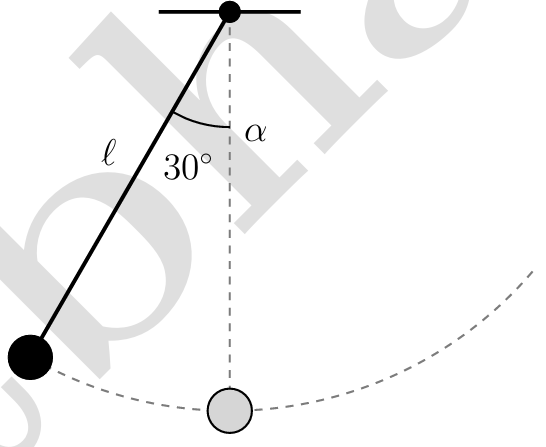
\includegraphics[width=0.30\textwidth]{images/8/8-8.png}\hfill
  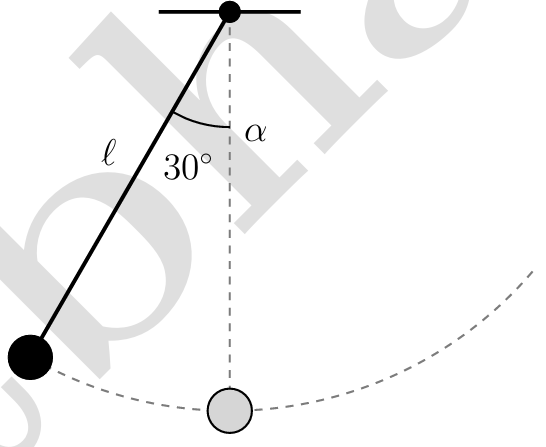
\includegraphics[width=0.30\textwidth]{images/8/8-9.png}
\end{center}
\begin{pilB}
  \item $4{,}31$ \item $6{,}69$ \item $48{,}49$ \item $2{,}39$ \item $7{,}43$
\end{pilB}
\end{soal}

\begin{soal}{20 \normalfont\small[Superposisi Getaran Harmonik]}
Dua getaran harmonik dengan frekuensi sudut yang sama dinyatakan oleh $y_1=6\sin20t$ dan
$y_2=8\cos20t$, dengan $y$ dalam cm dan $t$ dalam sekon. Jika resultannya ditulis sebagai
$y=R\sin(20t+\varphi)$, maka amplitudo resultan $R$ adalah \ldots
\begin{pilB}
  \item $14$~cm \item $12$~cm \item $10$~cm \item $8$~cm \item $2$~cm
\end{pilB}
\end{soal}

% ===================================================================
%  SOAL 21 -- 30
% ===================================================================

\begin{soal}{21 \normalfont\small[Efek Doppler pada Bunyi Pantul]}
Sebuah mobil pemadam bergerak menuju dinding sambil membunyikan sirene berfrekuensi
$680$~Hz. Pengemudi mendengar bunyi pantul dari dinding dengan frekuensi $760$~Hz. Jika
cepat rambat bunyi di udara $340$~m/s, kelajuan mobil pemadam adalah \ldots
\begin{pil}
  \item $54$~km/jam \item $60$~km/jam \item $68$~km/jam \item $72$~km/jam \item $90$~km/jam
\end{pil}
\end{soal}

\begin{soal}{22 \normalfont\small[Gerak Rotasi Diperlambat]}
Sebuah motor listrik yang dapat memutar roda dengan laju sudut $90$ putaran per menit
dimatikan dengan perlambatan sudut sebesar $2$~rad/s$^2$. Lama waktu yang diperlukan
roda tersebut untuk berhenti adalah \ldots~s.
\begin{pilB}
  \item $6{,}17$ \item $4{,}71$ \item $2{,}09$ \item $6{,}23$ \item $5{,}24$
\end{pilB}
\end{soal}

\begin{soal}{23 \normalfont\small[Susunan Pegas dan Frekuensi]}
Tiga pegas identik masing-masing berkonstanta $k$ disusun menjadi dua sistem. Sistem P
terdiri atas dua pegas yang disusun seri lalu diparalelkan dengan satu pegas. Sistem Q
terdiri atas dua pegas yang disusun paralel lalu diserikan dengan satu pegas. Kedua sistem
dipasangi massa yang sama $m$. Perbandingan frekuensi getar sistem P dan Q, yaitu
$f_P:f_Q$, adalah \ldots
\begin{pilB}
  \item $1:2$ \item $\sqrt{2}:1$ \item $3:2$ \item $2:3$ \item $1:\sqrt{2}$
\end{pilB}
\end{soal}

\begin{soal}{24 \normalfont\small[Cepat Rambat Bunyi dalam Fluida]}
Cepat rambat bunyi dalam fluida ideal memenuhi hubungan $v=\sqrt{B/\rho}$, dengan $B$
modulus bulk dan $\rho$ massa jenis fluida. Tinjau pernyataan berikut:
\begin{enumerate}[label=(\arabic*),leftmargin=*,topsep=2pt,itemsep=1pt]
  \item Semakin besar modulus bulk, bunyi merambat semakin cepat.
  \item Untuk $B$ tetap, semakin besar massa jenis maka bunyi merambat semakin lambat.
  \item Tegangan permukaan merupakan besaran utama yang menentukan cepat rambat bunyi di
        seluruh fluida homogen.
  \item Fluida yang sukar dimampatkan cenderung memiliki cepat rambat bunyi lebih besar.
\end{enumerate}
Pernyataan yang benar adalah \ldots
\begin{pil}
  \item (1) dan (2)
  \item (1), (2), dan (4)
  \item (2) dan (3)
  \item (3) dan (4)
  \item (1), (2), (3), dan (4)
\end{pil}
\end{soal}

\begin{soal}{25 \normalfont\small[Pusat Massa Empat Benda]}
Tinjau empat benda bermassa sama, dinamakan benda 1, 2, 3, dan 4. Benda $n$ ($n=1,2,3,4$)
bergerak dengan vektor posisi $\vec{r}_n(t)=\dfrac{n}{2}\vec{v}+\vec{a}\,t$. Jika
$\vec{v}=(4\hat{i}+2\hat{j})$~m/s, $\vec{a}=-5\hat{j}$~m/s$^2$, dan pada $t=0$ s keempat
benda berada di pusat koordinat, vektor posisi pusat massa sistem pada saat $t=1$~s
adalah \ldots~m.
\begin{pil}
  \item $2\hat{i}-4\hat{j}$
  \item $5\hat{i}-2{,}5\hat{j}$
  \item $1{,}5\hat{i}-4{,}25\hat{j}$
  \item $2{,}5\hat{i}-3{,}75\hat{j}$
  \item $0{,}5\hat{i}-4{,}75\hat{j}$
\end{pil}
\end{soal}

\begin{soal}{26 \normalfont\small[Efek Doppler Pengamat Menjauh]}
Sebuah drone diam membunyikan alarm berfrekuensi $500$~Hz. Seorang pelari bergerak
menjauhi drone dengan kelajuan $10$~m/s. Jika cepat rambat bunyi di udara $340$~m/s,
frekuensi yang didengar pelari adalah \ldots
\begin{pilB}
  \item $470{,}6$~Hz \item $485{,}3$~Hz \item $500{,}0$~Hz \item $514{,}7$~Hz \item $529{,}4$~Hz
\end{pilB}
\end{soal}

\begin{soal}{27 \normalfont\small[Periode Osilasi dari Energi Potensial]}
Sebuah benda bermassa $2$~kg berosilasi harmonik sederhana pada pegas licin. Energi
potensial sistem terhadap simpangan memenuhi hubungan $U=25x^2$, dengan $U$ dalam joule
dan $x$ dalam meter. Periode osilasi benda tersebut adalah \ldots
\begin{pil}
  \item $\dfrac{\pi}{10}$~s \item $\dfrac{\pi}{5}$~s \item $\dfrac{\pi}{\sqrt{2}}$~s
  \item $\dfrac{2\pi}{5}$~s \item $\pi$~s
\end{pil}
\end{soal}

\begin{soal}{28 \normalfont\small[Pernyataan tentang Getaran Pegas]}
Sebuah pegas yang dibebani bergetar vertikal sebanyak $15$ kali dalam $12$~sekon.
Tinjau pernyataan berikut:
\begin{enumerate}[label=(\arabic*),leftmargin=*,topsep=2pt,itemsep=1pt]
  \item Periode getaran adalah $0{,}8$~s.
  \item Frekuensi getaran adalah $1{,}25$~Hz.
  \item Waktu dari titik setimbang ke simpangan maksimum adalah $0{,}20$~s.
  \item Percepatan maksimum terjadi saat beban berada di titik setimbang.
\end{enumerate}
Pernyataan yang benar adalah \ldots
\begin{pil}
  \item (1), (2), dan (3)
  \item (1) dan (3)
  \item (2) dan (4)
  \item (4) saja
  \item (1), (2), (3), dan (4)
\end{pil}
\end{soal}

\begin{soal}{29 \normalfont\small[Tegangan Tali dari Persamaan Gelombang]}
Sebuah gelombang transversal pada tali dinyatakan oleh $y=0{,}04\sin(\pi x-40\pi t)$,
dengan $x$ dan $y$ dalam meter serta $t$ dalam sekon. Jika massa jenis linear tali adalah
$2\times10^{-3}$~kg/m, maka tegangan tali adalah \ldots
\begin{pilB}
  \item $1{,}6$~N \item $2{,}4$~N \item $3{,}2$~N \item $4{,}0$~N \item $6{,}4$~N
\end{pilB}
\end{soal}

\begin{soal}{30 \normalfont\small[Usaha dan Energi pada Bidang Miring Licin]}
Sebuah balok bermassa $4$~kg ditarik menggunakan gaya konstan $24$~N sejajar dengan
permukaan bidang miring licin yang membentuk sudut $30^\circ$ terhadap horizontal.
Balok dimulai dari keadaan tak bergerak. Kelajuan balok setelah mendaki bidang miring
sejauh $2$~m adalah \ldots~m/s.
\begin{pilB}
  \item $2{,}83$ \item $2{,}00$ \item $4{,}00$ \item $5{,}66$ \item $3{,}74$
\end{pilB}
\end{soal}

\end{document}
